\documentclass[twocolumn]{article}[10pt]
\usepackage[english]{babel} 
\usepackage[latin1]{inputenc} 
\usepackage{times} 			% Default times font style
\usepackage[T1]{fontenc} 	% Font encoding
\usepackage{amsmath} 		% Math package
\usepackage{mathtools} 		% Adds the declare paired 
							% delimeter command to make costom \abs and \norm
\usepackage{breqn}		 	% Adds dmath environment for automated brakeline
\usepackage{xfrac}			% Adds slanted fractions (sfrac)
\usepackage{cancel}			% Adds the cancel command, a slash through the symbol(s)
\usepackage{tabularx}		% Adds adjustable width on tabulars
\usepackage{cuted}			% Adds the strip command, pagewidth text in a twocolumn
							% environment. 
\usepackage{hyperref}
\usepackage{xcolor}
\usepackage{graphicx}

\linespread{1.1} 			% Two column layout can make blocks of text very dense. 

% Start costum \abs \norm 
\DeclarePairedDelimiter\abs{\lvert}{\rvert}%
\DeclarePairedDelimiter\norm{\lVert}{\rVert}%
% Swap the definition of \abs* and \norm*, so that \abs
% and \norm resizes the size of the brackets, and the 
% starred version does not.
\makeatletter
\let\oldabs\abs
\def\abs{\@ifstar{\oldabs}{\oldabs*}}
%
\let\oldnorm\norm
\def\norm{\@ifstar{\oldnorm}{\oldnorm*}}
\makeatother
% End costum \abs \norm 

\title{Project FYS4130}

\begin{document}
\maketitle
{\center \section*{Part 1}}
{\color{black!70}
1. Calculate $\langle X^2\rangle$ for both correlated and uncorrelated velocities by setting $p=1/2, p=1\%$ and $p=10\%$. Calculate the ensemble average with $10^5$ realizations and use $N = 1000$.
}

\begin{figure}
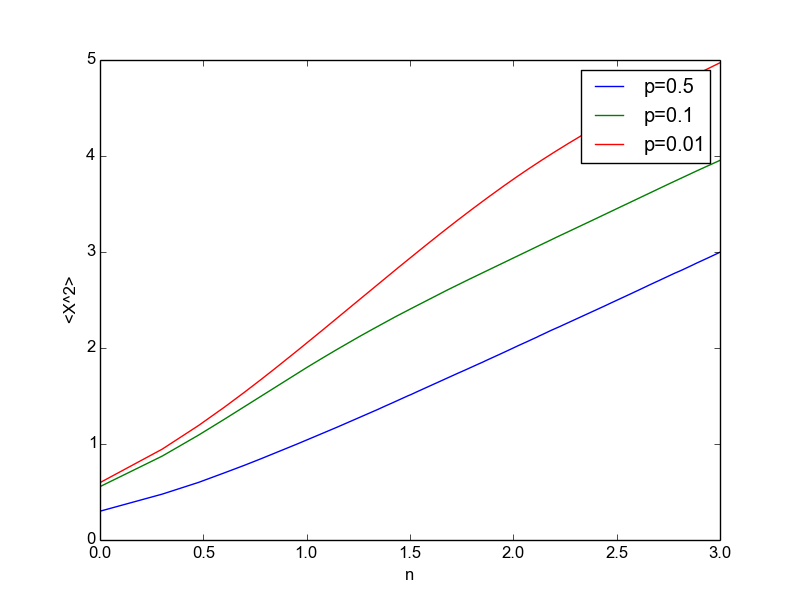
\includegraphics[width=0.50\textwidth]{part1_1.png}
\caption{$\langle X^2\rangle$ over $n$ steps. }
\label{fig:1}
\end{figure}

In figure \ref{fig:1} we can see the difference between the $p$ values.
Low values of $p$ makes the walker goes further. 


{\color{black!70}2. Make a logarithmic plot, i.e.e plot the variance 
$\log_{10}(\langle\Delta X^2 \rangle))$ as a function of $\log_{10}$ 
with $t = i$ and identify linear portions of the graphs. Discuss the 
corresponding early time exponents of $p=1\%$ and $p=10\%$ graphs and
why they change at later times. 
}
\begin{figure}
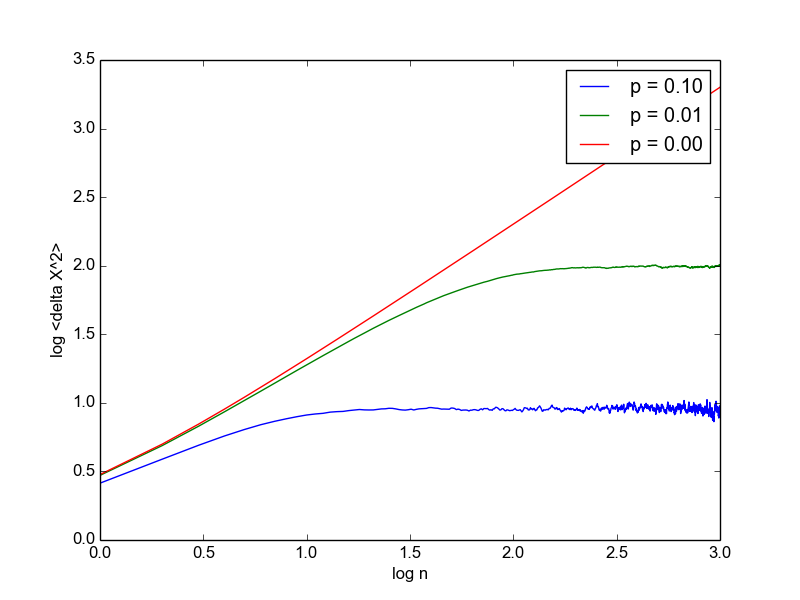
\includegraphics[width=0.50\textwidth]{part1_2.png}
\caption{$\langle \Delta X^2\rangle$ over $\log n$ }
\label{fig:2}
\end{figure}

Figure \ref{fig:2} shows $\log_{10}(\langle\Delta X^2 \rangle))$ for the two cases. 
By looking at $\langle X^2\rangle$ it is hard to interpret what is happening,
 but now we see clear plateaus. This suggest that after the walkers
has walked a certain amount of steps it stops moving and holds a mean 
position around this point. 

The function $n^2 - (n-1)^2 = 2n-1$ is also shown in the plot. This is to
compare the walkers to a walker which has no chance of turning around.
In this simple case the mentioned function is the analytical solution. 

Another way to interpret this is to say that the start of the plateu
is a kind of characteristic length for when the walker becomes a 
random walker with $p = 0.5$. The same plot for $p = 0.5$ are not shown
but only holds constant value at all steps. 

{\color{black!70} 3. For $p=0.5$, show that we may write 
$\langle\Delta X^2 \rangle = 2Dt$ and identify the value of $D$.
}

The average displacement of a random walker with equal probability 
to walk either directions is $0$. The variance is then simply
$\langle X(n)^2\rangle$. 
\begin{align*}
	\langle X(n)^2\rangle 
	&= 
	\left(\sum_i^n\Delta X_i\right)\left(\sum_j^n\Delta X_j\right)\\
	\langle X(n)^2\rangle 
	&= 
	\sum_i^n\Delta X_i^2 + \sum_{i\neq j}^n\Delta X_i\Delta X_j\\
	\langle X(n)^2\rangle 
	&= 
	l^2 n\\
\end{align*}
Where $\Delta X = \pm l$ is the steplength and $n$ is the number of steps. The non-diagonal contribution should be zero as long as the steps are not correlated. 

We can now relate this result to the variance from the diffusion equation by
defining 
\begin{align*}
n \equiv \frac{t}{\Delta t} && 2D \equiv \frac{l^2}{\Delta t}.
\end{align*}
\begin{align*}
\langle X(n)^2\rangle = 2Dt
\end{align*}
With the natural units $\Delta t = 1$ and $l = \pm1$, 
the value of $D$ will be $D = 1/2$.

{\color{black!70} 
4. If $X(t)$ is taken to be a description of the position of a molecule 
in a gas, then give a physical interpretation of the $p$-variations.
In particular, what state of the gas would small $p$ values 
correspond to?
}

Small $p$-values would correspond to a long mean displacement of a gas
molecule. Small $p$ makes it less likely that that particle will collide
into any other molecules in a given interval $\Delta t$. On the other 
side, high $p$-values would make it more likely that a molecule would
collide and change direction. This would be a high density system. 

The system is described by the probability of changing direction, $p$,
during a step $\Delta n$ but the number of steps in one timestep
$\Delta t$ is what decides the scale of the system. For instance,
if we defined $100\Delta t = \Delta n$ for our system at $p = 0.01$
, we can se that only one step would take us to the plateu. 

{\color{black!70} 
5. Make a histogram of the $X_N$-values to obtain the distribution 
$P(X)$ for $p=0.5$ and $p = 0.9$. Plot $\ln(P(X))$ as a function
of $X^2$ and use this to write down an analytic expression for
$P(X)$. Discuss the difference for the different $p$-values. 
}
\begin{figure}
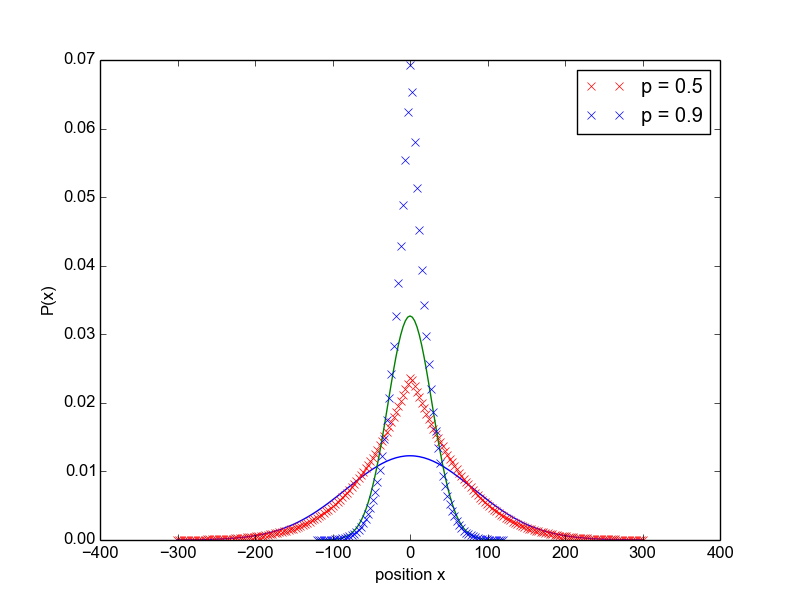
\includegraphics[width=0.50\textwidth]{part1_5_1.png}
\caption{Probability distribution $P(X)$}
\label{fig:3}
\end{figure}

Figure \ref{fig:3} shows the normalized probability distributions. 
The distribution for  $p=0.9$ has a smaller variance than 
$p=0.5$ because it changes directions often and we note
how both looks like normal distributions. Figure \ref{fig:4} shows
$\ln(P(X))$ over $X^2$. Straight lines suggest a distribution
on the form $$e^{-ax^2}.$$ The graphs are not straight in the
first parts, but when we make an analytical expression we
make this simplification. 
To make the expression we do a simple line fit, what we loose
in this simplification is the shart peak. 

\begin{figure}
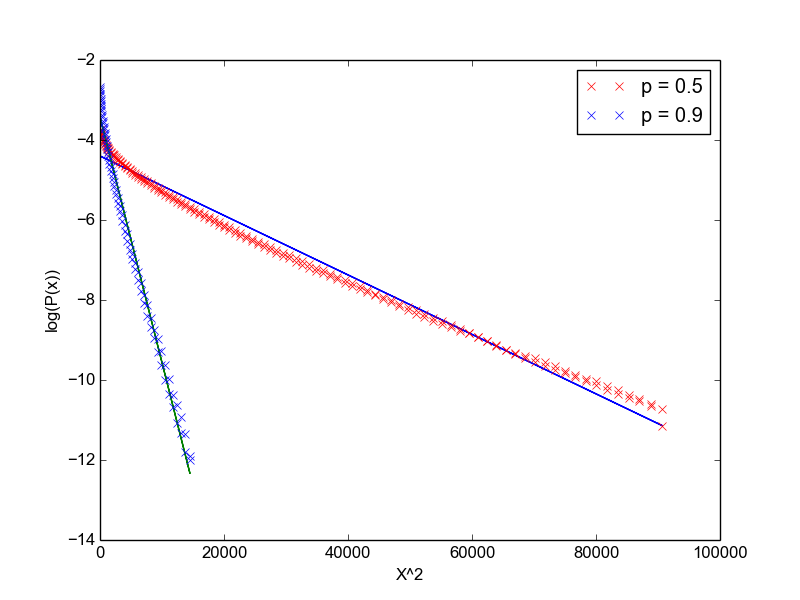
\includegraphics[width=0.50\textwidth]{part1_5_2.png}
\caption{Probability distribution $\log P(X)$ over $X^2$}
\label{fig:4}
\end{figure}

{\color{black!70} 
6. Use the analytic expression of $P(x)$ to calculate 
$\langle X^2(t)\rangle = \int x^2 P(x)\,dx /\int dx P(x)$. 
Use this to express in terms of D int the $p=0.5$ case. Obtain a 
from the histogram and compare the values of $D$.
}

The values for $a$ was estimated to $a_{p=0.5}=7.43\cdot 10^{-5}$
If we evalue the forementioned expression we get 
\begin{align*}
\langle X^2(t)\rangle 
&= 
\int_{-\infty}^\infty x^2 P(x)\,dx /\int_{-\infty}^\infty dx P(x)\\
Dt&=\frac{1}{2a^3}.
\end{align*}
$t$ in this case would be the number of steps if we set $\Delta t = 1$. 
If we evalute this I do not get a reasonable value for $D$. The above
integral does account for normalization which I also did in my program
and the value of $a$ does fit appropriately. Not sure what went wrong. 

{\center \section*{Part 2}}
{\color{black!70} 
We shall study the black body radiation field in a fictituous 2 
dimensional world. The expression in equation (5.38) in the text 
book is still valid in this case. 

1. Assuming periodic boundary conditions, how must the wave numbers
$k_x$ and $k_y$ be quantizied?
}

In the case of $\psi_n(0) = 0$ and 
$\psi_n(L) = 0$ we can easily calculate the wave numbers to be
\begin{align*}
k_i = \frac{n_i\pi}{L}&& n_i=0,1,2,3,\dots,N.
\end{align*}
With periodic boundries $\psi_n(x) = \psi_n(x + L)$ we get
\begin{align*}
k_i = \frac{2n_i\pi}{L}&& n_i= 0, \pm1,\pm2,\pm3,,\dots,\frac{N}{2}.
\end{align*}
because we now demand that the function is equal to itself at
a constant distance. Now it is important to include negative values
of $k$ to avoid under counting. This is easy to understand if we 
remember the rule $$\sin(-kx) = -\sin(kx).$$

{\color{black!70} 
2. Calculate the internal energy of the field $U(T)$ and the corresponding
capacity. 
}

We have:
\begin{align*}
\langle \epsilon_{\mathbf k}\rangle = \frac{\hbar\omega}{e^{\hbar\omega/kT}-1}
&&
U(T) = 2\sum_{\mathbf k} \langle \epsilon_{\mathbf k}\rangle 
\end{align*}
Now we turn the sum into an integral. 
We have to remember to add a factor $1/(2\pi)^2$ in the integral. 

\begin{align*}
U(T) = 2A\int \frac{d^2k}{(2\pi)^2} \frac{\hbar\omega}{e^{\hbar\omega/kT}-1}\\
U(T) = \frac{A}{c^2\pi}\int_0^\infty \omega \frac{\hbar\omega}{e^{\hbar\omega/kT}-1}d\omega
\end{align*}
In the second step we use the relation $d^2k = \frac{1}{c^2}2\pi\omega d\omega$. 
This we get from counting the discrete $k_x$ and $k_y$ in an area from 
$\omega$ to $\omega + d\omega$ on a disc 
instead of a sphere in the case of 3 dimentions. 

\begin{align*}
U(T) = \frac{A}{c^2\pi}\int_0^\infty \omega \frac{\hbar\omega}{e^{\hbar\omega/kT}-1}d\omega\\
U(T) = \frac{A\hbar}{c^2\pi}\left(\frac{kT}{\hbar}\right)^3
	\int_0^\infty \frac{x^2}{e^{x}-1}dx\\
U(T) = \frac{A\hbar}{c^2\pi}\left(\frac{kT}{\hbar}\right)^3
	2!\zeta(2+1)\\
U(T) \approx 2\frac{A\hbar}{c^2\pi}\left(\frac{kT}{\hbar}\right)^3
	\frac65
\end{align*}
In the last step we do the approximation $\zeta(3) = \frac65$ because 
there seems that zeta function is not nicely defined at this value. 
Now the heat capacity is $$C_v = \frac{\partial U}{\partial T},$$ which means
the heat capacity will go as $C_v\propto T^2$ in the 2 dimentional case. 

\newpage
(You must excuse my loose integration as factors are
very easily missed and they seem to magically appear and disappear
at different instances.)


















\end{document}